\documentclass{article}
\usepackage{multicol}
\usepackage{caption}
\usepackage{graphicx}
\usepackage{tabularx}
\usepackage{hyperref}

\newenvironment{Figure}
  {\par\medskip\noindent\minipage{\linewidth}}
  {\endminipage\par\medskip}
\begin{document}

\title{Distributed Llama - Distributed Inference of Large Language Models with Slow Synchronization over Ethernet}
\date{2024}
\author{Bartłomiej Tadych\\\small{bartlomiej.tadych@gmail.com}}

\maketitle

\begin{abstract}

Distributed Llama is a system designed to distribute the inference of large language models using readily available home devices. By distributing computation and weights across multiple devices, the system achieves accelerated inference with each additional device integrated into the system. This approach optimizes the utilization of resources for enhanced performance.

\end{abstract}

\begin{multicols}{2}

\section{Introduction}

Large language models (LLMs) require a significant amount of memory. For most home computers, running the inference of such large models is unfeasible. Although quantization mitigates this problem to some extent, very large models are still unattainable for home use. For example, Llama 2 \cite{llama2}  with 70 billion parameters, quantized to Q40 format, requires a minimum of 36.98GB of memory.

Projects such as Petals \cite{borzunov2022petals} or Llama.cpp MPI \cite{llamacpp} enable the execution of Large Language Models (LLMs) across multiple devices by partitioning neural network layers. This division distributes the memory requirements among all devices, but the drawback is that devices do not operate in parallel; each device processes only its assigned layers. Consequently, calculations occur sequentially, with only one device performing computations at a time, while the others wait for the results of the preceding one.

\begin{Figure}
  \centering
  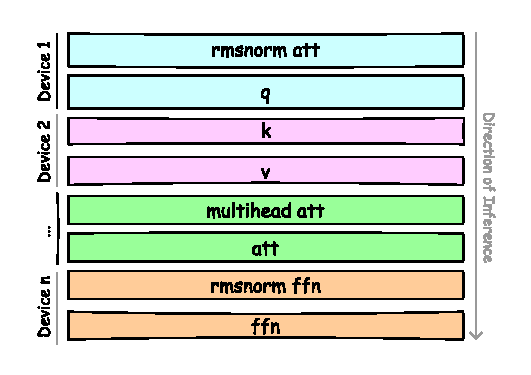
\includegraphics[width=\linewidth]{fig1.pdf}
  \captionof{figure}{Layer division using Petals or Llama.cpp MPI; each color represents a separate device.}
\end{Figure}

Distributed Llama addresses these challenges by introducing an alternative method to partition Large Language Models (LLMs). In this system, the model is vertically divided, where each device receives nearly all layers but is responsible only for forwarding its designated fragment of the layer. Additionally, each device retains in memory only the weights necessary for forwarding the assigned fragment. Since certain LLM layers demand the complete output from the preceding layer, Distributed Llama consolidates outputs and synchronizes all devices.

\begin{Figure}
  \centering
  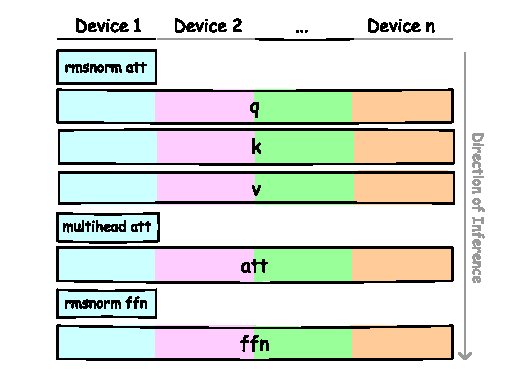
\includegraphics[width=\linewidth]{fig2.pdf}
  \captionof{figure}{Layer division using\\ Distributed Llama; each color represents a separate device.}
\end{Figure}

Some layers were not parallelized across multiple devices because the computational workload was too small, or the data to be synchronized was too large to justify the benefits of parallelization. Consequently, one device processes a slightly greater number of layers and requires slightly more memory than the others. We designate this device as the root device.

Distributed Llama supports weight quantization to reduce memory requirements. Additionally, it supports the quantization of data required for synchronization, significantly reducing the amount of information needed to be transferred across devices.

\section{Tests}

To test this approach I chose 8 Raspberry PI 4B 8GB devices connected together via Gigabit Ethernet to TP-Link LS1008G Switch. Raspberry PI 4B has quite slow 1500 Mhz processor and only 4 cores but it’s enough to observe how the new approach behaves when increasing the number of devices in the system. All tests were performed on quantized weights to Q40 format and quantized synchronization data to Q80 format.

\end{multicols}

\vspace{10pt}

\begin{Figure}
  \noindent\begin{tabularx}{\columnwidth} { 
    >{\arraybackslash\hsize=7.5\hsize}X
    | >{\arraybackslash\hsize=5\hsize}X
    | >{\arraybackslash\hsize=5\hsize}X
    | >{\arraybackslash\hsize=5\hsize}X
    | >{\arraybackslash\hsize=5.5\hsize}X}
  Llama 2 7B & 1 Device & 2 Devices & 4 Devices & 8 Devices \\
  \hline
  Total & 1312.50 ms & 793.69 ms & \textbf{494.00 ms} & 588.19 ms \\
  \hline
  Inference & 1307.94 ms & 739.00 ms & 458.81 ms & 296.69 ms \\
  \hline
  Synchronization & 1.81 ms & 52.50 ms & 34.06 ms & 289.75 ms \\
  \end{tabularx}
  \captionof{figure}{Single-token generation time for the Llama 2 7B model on Raspberry Pi 4B 8GB devices. Number of samples: 16.}
\end{Figure}

\begin{Figure}
  \noindent\begin{tabularx}{\columnwidth} { 
    >{\arraybackslash\hsize=7.5\hsize}X
    | >{\arraybackslash\hsize=5\hsize}X
    | >{\arraybackslash\hsize=5\hsize}X
    | >{\arraybackslash\hsize=5\hsize}X
    | >{\arraybackslash\hsize=5.5\hsize}X}
  Llama 2 13B & 1 Device & 2 Devices & 4 Devices & 8 Devices \\
  \hline
  Total & - & 1497.19 ms & \textbf{848.19 ms} & 1114.88 ms \\
  \hline
  Inference &- & 1465.06 ms & 746.88 ms & 460.8 ms \\
  \hline
  Synchronization & - & 30.88 ms & 99.50 ms & 652.88 ms \\
  \end{tabularx}
  \captionof{figure}{Single-token generation time for the Llama 2 13B model on Raspberry Pi 4B 8GB devices. Generation on single device was not possible due to memory limitations. Number of samples: 16.}
\end{Figure}

\begin{Figure}
  \noindent\begin{tabularx}{\columnwidth} { 
    >{\arraybackslash\hsize=7.5\hsize}X
    | >{\arraybackslash\hsize=5\hsize}X
    | >{\arraybackslash\hsize=5\hsize}X
    | >{\arraybackslash\hsize=5\hsize}X
    | >{\arraybackslash\hsize=5.5\hsize}X}
  Llama 2 70B & 1 Device & 2 Devices & 4 Devices & 8 Devices \\
  \hline
  Total & - & - & - & \textbf{4842.81 ms} \\
  \hline
  Inference & - & - & - & 2121.94 ms \\
  \hline
  Synchronization & - & - & - & 2719.62 ms\\
  \end{tabularx}
  \captionof{figure}{Single-token generation time for the Llama 2 70B model on Raspberry Pi 4B 8GB devices. Generation was possible only on 8 devices due to memory limitations. Number of samples: 16.}
\end{Figure}

\begin{Figure}
  \noindent\begin{tabularx}{\columnwidth} { 
    >{\arraybackslash\hsize=10\hsize}X
    | >{\arraybackslash\hsize=6\hsize}X
    | >{\arraybackslash\hsize=6\hsize}X
    | >{\arraybackslash\hsize=6\hsize}X}
  Model & 2 Devices & 4 Devices & 8 Devices \\
  \hline
  Llama 2 7B & 1112 kB & 2830 kB & 6008 kB \\
  \hline 
  Llama 2 13B & 1742 kB & 4430 kB & 9407 kB \\
  \hline
  Llama 2 70B & - & - & 32873 kB \\
  \end{tabularx}
  \captionof{figure}{The amount of data required to synchronize devices for generating one token. The transferred data was quantized to Q80 format.}
\end{Figure}

\begin{multicols}{2}

\section{Discussion}

Generating a single token requires minimal data for synchronization compared to the overall size of the model. As the number of devices increases, the data needed for synchronization also grows, leading to a slowdown in inference. However, despite this challenge, a significant improvement in inference speed is observed in direct proportion to the number of devices in the system, aligning with the project's overarching goal.

Synchronization tests were conducted on a slow Gigabit Ethernet link. The speed of this link significantly influences the final results. For instance, the inference time of Llama 2 70B is faster than the synchronization time. Using a faster link will result in a greater benefit from distributed computing.

\emph{Future work:} The described approach can also be applied to distributed learning of LLMs, enabling accelerated learning speeds through the utilization of multiple devices.

\end{multicols}

\begin{thebibliography}{9}
  \bibitem{llama2}
  Hugo Touvron and Louis Martin and Kevin Stone and Peter Albert and Amjad Almahairi and Yasmine Babaei and Nikolay Bashlykov and Soumya Batra and Prajjwal Bhargava and Shruti Bhosale and Dan Bikel and Lukas Blecher and Cristian Canton Ferrer and Moya Chen and Guillem Cucurull and David Esiobu and Jude Fernandes and Jeremy Fu and Wenyin Fu and Brian Fuller and Cynthia Gao and Vedanuj Goswami and Naman Goyal and Anthony Hartshorn and Saghar Hosseini and Rui Hou and Hakan Inan and Marcin Kardas and Viktor Kerkez and Madian Khabsa and Isabel Kloumann and Artem Korenev and Punit Singh Koura and Marie-Anne Lachaux and Thibaut Lavril and Jenya Lee and Diana Liskovich and Yinghai Lu and Yuning Mao and Xavier Martinet and Todor Mihaylov and Pushkar Mishra and Igor Molybog and Yixin Nie and Andrew Poulton and Jeremy Reizenstein and Rashi Rungta and Kalyan Saladi and Alan Schelten and Ruan Silva and Eric Michael Smith and Ranjan Subramanian and Xiaoqing Ellen Tan and Binh Tang and Ross Taylor and Adina Williams and Jian Xiang Kuan and Puxin Xu and Zheng Yan and Iliyan Zarov and Yuchen Zhang and Angela Fan and Melanie Kambadur and Sharan Narang and Aurelien Rodriguez and Robert Stojnic and Sergey Edunov and Thomas Scialom (2023) Llama 2: Open Foundation and Fine-Tuned Chat Models, arXiv:2307.09288

  \bibitem{borzunov2022petals}
  Borzunov, Alexander and Baranchuk, Dmitry and Dettmers, Tim and Ryabinin, Max and Belkada, Younes and Chumachenko, Artem and Samygin, Pavel and Raffel, Colin (2022) Petals: Collaborative Inference and Fine-tuning of Large Models, arXiv:2209.01188

  \bibitem{llamacpp}
  Llama.cpp, \url{https://github.com/ggerganov/llama.cpp}, 20 Jan 2024
\end{thebibliography}

\end{document}
